\section{Experiment with Pozyx}
We have created an experiment to test how accurate the tags in Pozyx are.
The primary goal of the experiment was to test the accuracy, but a biproduct of the experiment was to see how many update frequencies there were with each tag.


\subsection{Setup}
The current settings goes for best precision, but gives a smaller amount of updates.
% Uddyb hvilke settings det er.
The setup of the experiment as seen on \autoref{fig:experiment-setup}. 
The experiment was conducted indoors in Novi 9. 
\texttt{0x632b} and \texttt{0x676e} was mounted on a wall 240 centimeters apart.
\texttt{0x6738} and \texttt{0x676c} was mounted on a bulletin board.
There was chosen different heights as Pozyx documentation suggests that not all anchors should have the same height.
%uddyb

\begin{figure}[H]
    \centering
    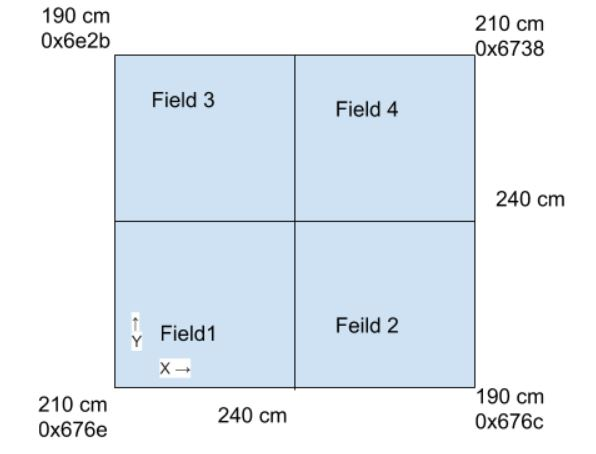
\includegraphics[width=0.6\linewidth]{experiment-setup.JPG}
    \caption{The setup of the experiment with the anchors and the height in the corners.}
    \label{fig:experiment-setup}
\end{figure}
\noindent
The fields was a blackboard where lines were drawn for each 10 centimeters to know the actual position as seen on.

\begin{figure}[H]
    \centering
    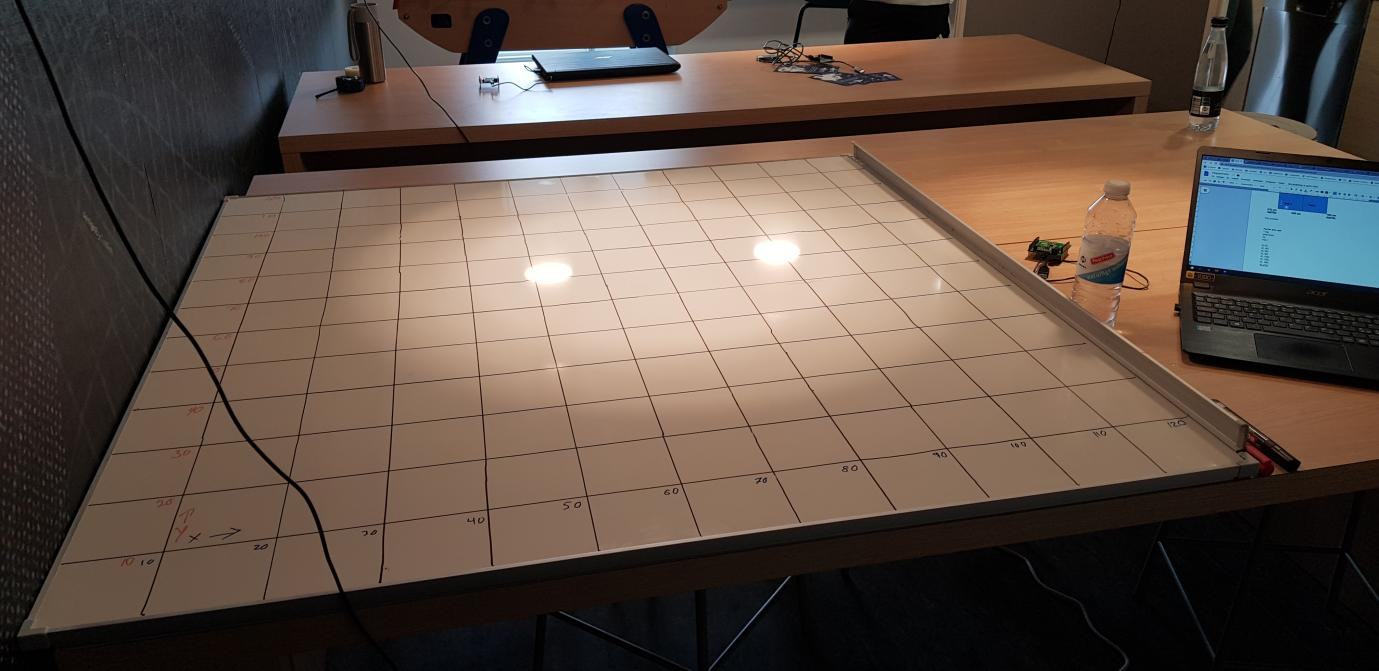
\includegraphics[width=0.8\linewidth]{experiment-blackboard.png}
    \caption{The blackboard with the drawn positions.}
    \label{fig:experiment-blackboard}
\end{figure}
 
\subsection{Precision with 1 tag}

\paragraph{Update frequency}

\subsection{Precision with 3 tag}

\paragraph{Update frequency}

\subsection{Precision with 5 tag}

\paragraph{Update frequency}

\subsection{Possible influences on the test}
Metal in the blackboard, especially at 120 cm.
Close to the wall


